\chapter{Phenomenological Framework for LHC Observables, Searches and Analysis}

Since its formulation, the Standard Model (SM) has proven remarkably successful in describing the fundamental particles and interactions, and its parameters have been measured with increasing precision over several decades; however, as we have commented in the last chapter, various theoretical and experimental observations suggest that the SM is incomplete and certain details of the standard model seem to demand a better explanation, motivating the exploration of new physics (NP) beyond the standard model (BSM) and in turn methods in the search for this new physics. This pursuit requires both the development of theoretical models and the design of experimental strategies to test them. Particle physics phenomenology plays a crucial role in this endeavor by bridging theoretical predictions with experimental observations, feasibility and searches, particularly in high-energy experiments such as those conducted at the Large Hadron Collider (LHC), as well as in high-precision low-energy measurements.

The LHC is a proton-proton ($pp$) collider that has been operating since 2009, achieving center-of-mass collision energies ranging from $7~\mathrm{TeV}$ to $13.6~\mathrm{TeV}$. During its Run~I~(2010-2013), the LHC reached $7~\mathrm{TeV}$ in 2010-2011 and $8~\mathrm{TeV}$ in 2012, leading to landmark discoveries such as the Higgs boson in 2012. Run~II~(2015-2018) operated at $13~\mathrm{TeV}$ and achieved an instantaneous luminosity of $1.5 \times 10^{34}~\mathrm{cm}^{-2}~\mathrm{s}^{-1}$, yielding approximately 1000 top-quark pairs and 50 Higgs bosons per minute. Run~III~(2022-2025) is currently underway with collisions at a record energy of $13.6~\mathrm{TeV}$ and even higher luminosities. Following this, the High-Luminosity LHC (HL-LHC) is expected to begin operations around 2029. This major upgrade aims to increase the integrated luminosity by more than an order of magnitude, targeting up to $3\,\mathrm{ab}^{-1}$ of data per experiment. The HL-LHC will significantly enhance the sensitivity to rare processes, improve the precision of Standard Model measurements, and boost the discovery potential for BSM phenomena.

These collisions take place at four main interaction points, each equipped with a sophisticated particle detector designed to record and analyze the outcomes. Two of the largest and most comprehensive experiments at the LHC are the Compact Muon Solenoid (CMS) and ATLAS detectors. Both are multipurpose detectors with broad physics programs, designed to explore a wide range of phenomena. They perform precision measurements within the electroweak sector of the SM, investigate the dynamics of quarks and gluons (including through heavy-ion collisions), and carry out extensive searches for BSM signatures using $pp$ collision data. While CMS and ATLAS differ in their detector designs and reconstruction strategies, their physics goals are largely overlapping, and their results are complementary. Throughout this work, phenomenological studies and comparisons are primarily developed in the context of CMS, although several results from ATLAS are also referenced, given the close alignment in sensitivity and scope.

\section{Coordinate System and Collision Parameters}
To fully describe the CMS experiment, some of its parameters should be outlined. Measurements performed at CMS adopt the coordinate system whose origin lies at the collision point, with the $y$-axis pointing vertically upward, the $x$-axis pointing radially inward towards the centre of the LHC and the $z$-axis along the beam direction. The azimuthal angle $\phi$ is measured in the $x y$-plane from the $x$-axis and the polar angle, $\theta$, is measured from the $z$-axis, as shown in the Fig.~\ref{fig_coordinates}. 
\begin{center}
	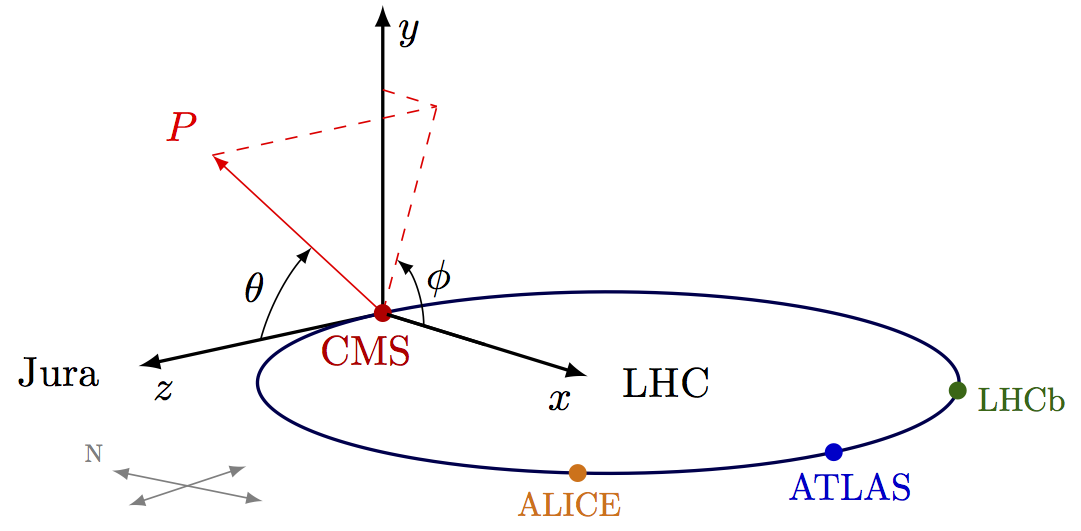
\includegraphics[width=0.8\textwidth]{Images/coordinatechart.png}
	\captionof{figure}{Coordinate system employed by the CMS experiment (retrieved from~\parencite{cmsplots}).}\label{fig_coordinates}
\end{center}

The event rate $R$ for a physical process (e.g., $pp \to X$) is governed by the accelerator's luminosity $\mathcal{L}$ and the process cross section $\sigma$. Luminosity quantifies the performance of a collider to produce interactions, establishing the proportionality,
\begin{equation}
	\frac{d R}{d t} = \mathcal{L} \sigma,
\end{equation}
where $\sigma$ (typically measured in barns, $1\,\text{b} = 10^{-24}\,\text{cm}^2$) encodes the interaction probability. For LHC proton bunches colliding head-on with Gaussian transverse profiles, the instantaneous luminosity is~\parencite{Herr:941318,book:1123430}:
\begin{equation}
	\mathcal{L} = \frac{f N_{b}}{4\pi} \frac{N_{1} N_{2}}{\sigma_{x} \sigma_{y}}\label{eq_lumi}
\end{equation}
Here, $N_{1,2}$ are proton counts per bunch, $f$ is the bunch collision frequency, $N_{b}$ is the number of bunches, and $\sigma_{x,y}$ are transverse beam widths. 

Integrating $\mathcal{L}$ over time yields the total integrated luminosity $L$, linking directly to the observed event count $N$:
\begin{equation}
	L = \int \mathcal{L}\, dt \quad \Rightarrow \quad N = L \sigma.
\end{equation}
%At Run~II luminosities ($\mathcal{L} \approx 1.5 \times 10^{34}\,\text{cm}^{-2}\text{s}^{-1}$), a $1\,\text{pb}$ cross section produces $\sim\!15$ events per second. This framework underpins all LHC physics analyses, from Higgs measurements ($\sigma_{pp\to H} \sim 50\,\text{pb}$ at $13\,\text{TeV}$) to BSM searches for rare processes ($\sigma_{\text{BSM}} \ll 1\,\text{fb}$).
  
The Gaussian beam approximation in~\eqref{eq_lumi} ignores hourglass effects (beam divergence near interaction points) and dynamic $\sigma_{x,y}$ variations during fills. CMS mitigates these via real-time luminosity monitoring using pixel clusters~\parencite{Sirunyan2021}, with systematic uncertainties below $2\%$. High $\mathcal{L}$ also introduces pileup—multiple $pp$ interactions per bunch crossing—which complicates $\eta$/$\phi$ measurements but is corrected using vertex isolation algorithms.

\begin{center}
  		% CMS detector - left perspective
		\tdplotsetmaincoords{75}{50} % to reset previous setting
		\begin{tikzpicture}[scale=2.6,tdplot_main_coords,rotate around x=90]
			
			% VARIABLES
			\def\rvec{\L/2/cos(\thetavec)}
			\def\thetavec{18}
			\def\phivec{60}
			\def\L{3.3}    % detector length
			\def\R{0.75}   % detector cylinder radius
			\def\l{4.3}    % beam pipe length
			\def\r{0.04}   % beam pipe radius
			\def\rt{0.042} % beam pipe radius + line thickness
			\def\xmax{1}   % maximum x axis
			\def\ymax{1}   % maximum y axis
			\def\zmin{-\l/2-0.2} % minimum z axis
			\def\zmax{\l/2+0.3}  % maximum z axis
			\def\w{0.3}
			\coordinate (O) at (0,0,0);
			\coordinate (Z) at (0,0,\L/2);
			\tdplotsetcoord{O'}{0.022}{\thetavec}{\phivec} % slightly shifted origin
			\tdplotsetcoord{O''}{0.018}{90}{\phivec} % slightly shifted origin
			\tdplotsetcoord{P}{\rvec}{\thetavec}{\phivec}
			
			% CYLINDER behind
			\def\ang{19} % rotate lines to simulate cylinder
			\fill[top color=red!50!black!4,bottom color=red!60!black!2,rotate around z=\ang]
			(0,\R,\L/2) --++ (0,0,-\L) arc(90:270:\R) --++ (0,0,\L) arc(270:90:\R) -- cycle;
			\fill[detector surface] % transverse plane at z=L/2
			(0,0,\L/2) --++ (0,\R,0) arc(90:270:\R) -- cycle;
			\fill[detector surface] % transverse plane at z=-L/2
			(0,0,-\L/2) --++ (0,\R,0) arc(90:270:\R) -- cycle;
			\tdplotdrawarc[detector]{(0,0,\L/2)}{\R}{0}{360}{}{}
			\tdplotdrawarc[detector,thin]{(0,0,-\L/2)}{\R}{0}{360}{}{}
			%\draw[detector,canvas is yx plane at z=-\L/2] (0,0,0) circle(\R);
			\draw[detector,thin, dashed] % transverse plane at z=0
			(90-\ang:\R) arc (90-\ang:270:\R);
			\draw[detector] (0,0,-\L/2)++(90:\R) --++ (0,0,\L); % top horizontal
			\draw[detector] (0,0,-\L/2)++(-90:\R) --++ (0,0,\L); % bottom horizontal
			
			% BEAM PIPE
			\tdplotdrawarc[beam pipe]{(0,0,\l/2)}{\r}{0}{360}{}{}
			%\tdplotdrawarc[beam pipe]{(0,0,-\l/2)}{\r}{\ang-90}{90}{}{}
			%\draw[beam pipe] % cylindric beam pipe
			%  (0,\r,-\l/2) --++ (0,0,\l) arc(90:-90:\r)
			%  --++ (0,0,-\l) arc(-90:90:\r);
			\draw[beam pipe] % beam pipe, thinner in middle
			(0,\r,-\l/2) -- (0,\r,-0.2*\l) -- (90:0.5*\r)
			-- (0,\r,0.2*\l) -- (0,\r,0.5*\l) arc(90:-90:\r)
			-- (0,-\r,0.2*\l) -- (-90:0.5*\r) --
			(0,-\r,-0.2*\l) -- (0,-\r,-\l/2) arc(-90:90:\r);
			\draw[beam pipe] (0,0,\l/2) circle(\r);
			
			% AXES
			%\draw[thick,->] (0,0,0) -- (0,0,1) node[below right]{$z$}; % short
			\draw[axis,-] (0,0,\zmin) -- (0,0,0); % long
			\fill[CMScol] (O) circle(0.5pt) node[right=1,below=1] {IP};
			\draw[axis] (0,0,0.020) -- (0,0,\zmax) node[right=3,above=0.1]{$z$}; % long
			\draw[axis] (0,0.019,0) -- (0,\ymax,0) node[below left]{$y$};
			\draw[axis] (0.022,0,0) -- (\xmax,0,0) node[below=1,right=-2]{$x$};
			
			% LABELS
			\node[mydarkred,above] at (0,\ymax,0) {$\eta=0$};
			\node[mydarkred,above=0.6, left] at (0,\R,0.3*\L) {$\eta>0$};
			\node[mydarkred,above=0.7, right] at (0,\R,-0.2*\L) {$\eta<0$};
			\node[mydarkred,below=1,left] at (0,0,\zmax) {$\eta=\infty$};
			\node[mydarkred,above=1,right] at (0,0,\zmin) {$\eta=-\infty$};
			
			% VECTORS
			%\fill[radius=0.4,red] (P) circle;
			\draw[dashed,myred] (P)  -- (Pxy);
			\draw[dashed,myred] (Py) -- (Pxy);
			\draw[dashed,myred] (P) -- (Pz);
			
			
			\draw[->,miverde,line cap=round,draw opacity=0.9] (O') -- (P) node[anchor=-30] {\contour{white}{$\va*{p}$}};
			\draw[->,miverde,line cap=round] (O') -- (P) node[anchor=-30] {$\va*{p}$};
			
			\draw[->,azulF,line cap=round,draw opacity=0.9] (O') -- (Pxy) node[right, anchor=-100] {\contour{white}{$\va*{p}_T$}};
			% \draw[->,azulF,line cap=round] (O') -- (Pxy) node[right , anchor=-100] {$\va*{p}_T$};
			
			
			% CYLINDER front
			\draw[beam pipe,fill=none] (0,\r,-\l/2) arc(90:-90:\r);
			\fill[detector surface] % transverse plane at z=L/2
			(0,\rt,\L/2) --++ (0,\R-\rt,0) arc(90:-90:\R) --++ (0,\R-\rt,0) arc(-90:90:\rt);
			\fill[detector surface] % transverse plane at z=-L/2
			(0,\rt,-\L/2) --++ (0,\R-\rt,0) arc(90:-90:\R) --++ (0,\R-\rt,0) arc(-90:90:\rt);
			\tdplotdrawarc[detector]{(0,0,\L/2)}{\R}{-90}{90}{}{} % transverse plane at z=L/2
			\tdplotdrawarc[detector]{(0,0,-\L/2)}{\R}{-90}{90}{}{} % transverse plane at z=-L/2
			\draw[beam pipe,fill=none] (0,\r,\l/2) arc(90:-90:\r);
			\draw[detector,very thin, dashed] % transverse plane at z=0
			(90-\ang:\R) arc (90-\ang:-90:\R);
			
			% ANGLES
			\tdplotdrawarc[thick,red!57!black!3] % contour
			{(O)}{0.2}{4}{0.7*\phivec}{}{}

			% white to contour
			\tdplotdrawarc[draw=azulF, line width=0.6pt, draw opacity=0.9]{(O)}{0.2}{0}{\phivec}{above=2,right=0.75,anchor=-30,text=black}{\contour{white}{$\phi$}}
			\tdplotdrawarc[->, azulF]{(O)}{0.2}{0}{\phivec}{above=2,right=0.75,anchor=-30}{$\phi$}


			\tdplotdrawarc[->,rotate around z=\phivec-90,rotate around y=-90]
			{(O)}{0.88}{0}{\thetavec}{anchor=mid east}{$\theta$}
			\tdplotdrawarc[thick,red!58!black!4,rotate around z=\phivec-90,rotate around y=-90] % contour
			{(O)}{0.3}{88}{0.5*(90+\thetavec)}{}{}
			\tdplotdrawarc[-{>[flex'=1]},rotate around z=\phivec-90,rotate around y=-90,line cap=round]
			{(O)}{0.3}{90}{\thetavec}{above=4.5,right=0.5,anchor=mid east}{$\eta$}
			\draw[mydarkred] (0,0,\L/2) --++ (\R,0,0);
			\tdplotdrawarc[thick,red!60!black!6] % contour
			{(Z)}{0.2}{4}{0.7*\phivec}{}{}
			\tdplotdrawarc[draw=none,opacity=0.8]{(Z)}{0.2}{0}{\phivec}{above=2,right=0.7,anchor=-30}{\contour{red!60!black!6}{$\phi$}}
			\tdplotdrawarc[->]{(Z)}{0.2}{0}{\phivec}{above=2,right=0.7,anchor=-30}{$\phi$}
			
			% COMPASS - CMS-ATLAS axis has a ~12° declination (http://googlecompass.com)
			\begin{scope}[shift={(1.1*\R,-\R,0.2*\L)},rotate around y=12]
				\draw[<->,black!50] (-\w,0,0) -- (\w,0,0);
				\draw[<->,black!50] (0,0,-\w) -- (0,0,\w);
				\node[left,black!50,scale=0.6] at (-\w,0,0) {N};
				\node[below=3,left=-2,green!20!black!50,scale=0.6] at (0,0,\w) {Jura};
				%\node[below=1,right,black!50,scale=0.6,align=center] at (\w,0,0) {center of\\the LHC};
				%\node[below=1,right,blue!30!black!50,scale=0.6] at (\w,0,0) {ATLAS};
			\end{scope}
			\draw[->,thick,orange!30!black] (1.4*\w,-\R,-0.1*\L) --++ (2*\w,0,0)
			node[right,scale=0.8,align=center] {center of\\[-1pt]the LHC};
			
		\end{tikzpicture}
  \captionof{figure}{Detailed reparametrization of the coordinate system employed by the CMS experiment (retrieved from~\parencite{cmsplots})}\label{fig_cms_coor}
\end{center}
The following variables are related to the particles being produced rather than the accelerator.
\begin{description}
	\item[Decay width] ( $\Gamma)$ The decay rate is the probability that a given particle will decay per unit time. Since a particle can have multiple decay modes, the total decay rate is the sum of the decay rates for each mode~\parencite{book:1123430}. The relative frequency of a decay mode is the branching ratio, given by
	$$
	\mathrm{BR}(j)=\frac{\Gamma(j)}{\Gamma} .
	$$
	\item[Cross-section] $(\sigma)$ The cross-section is a measure of the probability that an interaction will occur from a collision. It is a quantum-mechanical analogue of the "effective size" of the particles involved in an interaction.

	\item[Pseudo-rapidity] $(\eta)$ Instead of using the polar angle, CMS measurements involve the pseudo-rapidity, defined by
	$$
	\eta=-\ln \left(\tan \frac{\theta}{2}\right)
	$$
	The main advantage of using the pseudo-rapidity is that distributions over it tend to be closer to a uniform distribution than those over the polar angle, see Fig.~\ref{fig_cms_coor}. Furthermore, the difference in pseudo-rapidity is invariant under Lorentz boosts along the beam direction~\parencite{book:1123430}.
	\item[Transverse Momentum] ($p_T$) Refers to the component of momentum which is perpendicular to the beam line. It is usually preferred over full momentum because momentum along the beamline may just be left over from the beam particles, while the transverse momentum is always associated with whatever physics happened at the vertex, see Fig.~\ref{fig_cms_coor}.
	\item[Missing transverse energy and momentum] $\left(E_{T}^{\text {miss }} \& p_{T}^{\text {miss }}\right)$ Missing energy and momentum refers to the energy and momentum that is not detected but is expected to be there as a consequence of energy conservation and momentum conservation. This momentum is often carried by particles that do not interact electromagnetically or strongly and are therefore difficult to detect~\parencite{book:1123430}. Missing energy and momentum provides an indirect measurement of undetectable particles in hadron colliders such as neutrinos. Missing momentum reconstructions focus on the transverse direction, where total momentum is expected to be zero.
\end{description}


\section{Detectors and Subsystems}

A typical collider experiment comprises several main detector subsystems that are used jointly to detect and measure the properties of particles produced in the collision. A \textit{schematic representation} of such a generic multipurpose detector is shown in Fig.~\ref{fig_detector}. The detector is typically composed of several concentric layers, each designed to measure different properties of the particles produced in the collisions. 

\begin{center}
	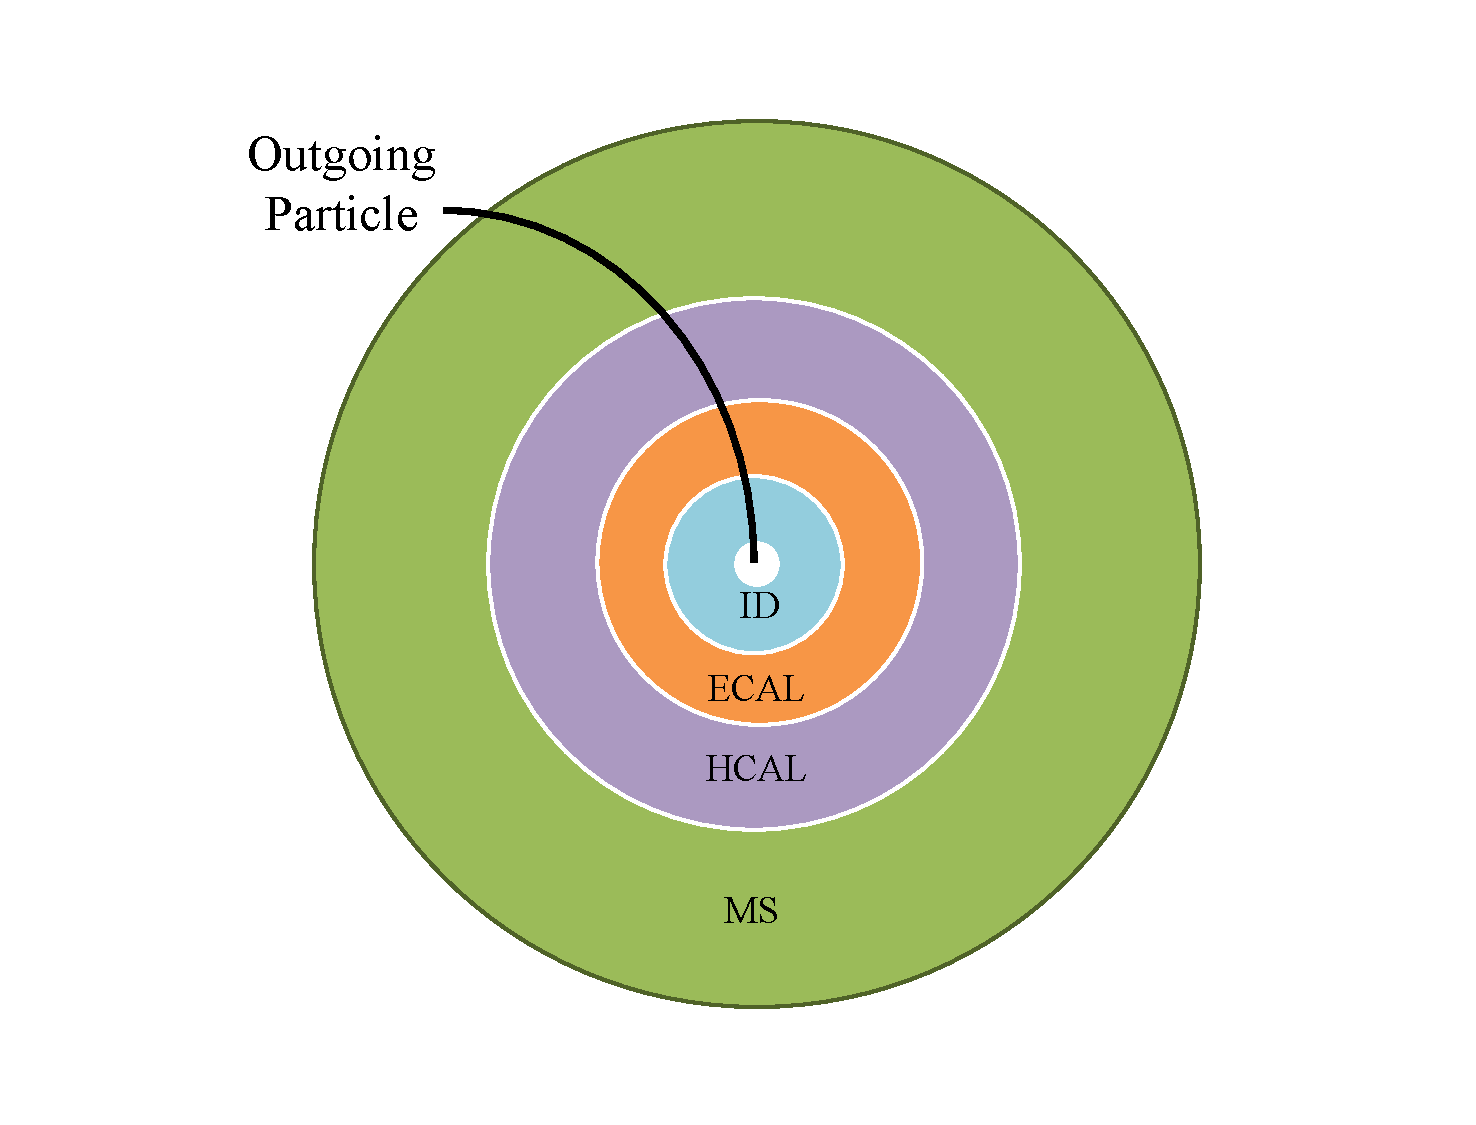
\includegraphics[width=0.8\textwidth]{Images/transversal_detector.pdf}
	\captionof{figure}{Schematic representation of transversal section of a generic multipurpose detector. The inner detector (ID) is used to measure the trajectories of charged particles, the electromagnetic calorimeter (ECAL) measures the energy of photons and electrons, the hadronic calorimeter (HCAL) measures the energy of hadrons, and the muon system (MS) measures the trajectories of muons. The missing transverse energy (MET) is measured by combining information from all subsystems..}\label{fig_detector}
\end{center}

The innermost subsystem, called the inner detector (ID), is designed to detect electrically charged particles that are long-lived enough to traverse the ID. The most common such particles from the SM are two charged leptons (the electron $e$ and the muon $\mu$ ) and three hadrons (the pion $\pi$, kaon $K$, and proton $p$ ). Regions of ionization produced by such a particle in solid-state or gaseous detector sensors are detected as spatial hits that are fit into a trajectory, referred to as a \textbf{track}. The direction and curvature of the track in a magnetic field yield the particle's momentum vector and electric charge. In some detectors, the ID is enclosed in a Cherenkov-light detector used to measure the velocity of the tracked particles. Combined with the momentum measurement in the ID, this yields the particle mass with sufficient resolution to differentiate between pions, kaons, and protons in a relevant momentum range.

After passing through the tracker, particles produced in the collisions typically enter an electromagnetic calorimeter (ECAL), designed to measure the energies of photons, electrons and positrons. The energy measurement exploits the properties of electromagnetic shower production via photon radiation and $e^{+} e^{-}$ pair production, resulting from the interaction of energetic particles with the ECAL material.

Hadrons deposit energy via hadronic interactions with the detector material. Since this process involves large fluctuations and a variety of energy-deposition mechanisms, precise hadron-energy measurement is achievable only at high-energy colliders, where fluctuations are effectively averaged out. In particular, high-energy quarks and gluons hadronize into a collimated spray of hadrons known as a \textbf{jet}. Containing the jet requires use of a deep hadronic calorimeter (HCAL) beyond the ECAL. While a jet can be identified solely in the calorimeters, its energy is nowadays measured from a combination of the momenta of tracks in the ID and the signals integrated in the ECAL and HCAL. 

The signals from the calorimeters, know as \textbf{towers}, are grouped into jets using a jet clustering algorithm. If and hadronic particle is neutral, it will not leave a track in the ID, but it will still deposit energy in the towers. So, the towers are used to measure the energy of neutral particles, such as photons and neutral hadrons, while the ID tracks are used to measure the energy of charged particles. This approach is known as particle flow (PF) reconstruction and provides a more accurate measurement of the energy of jets. 

Muons do not undergo hadronic interactions, and are heavy enough that they lose energy due to ionization at a low rate. Therefore, they lose only a few GeV while traversing a typical LHC-detector calorimeter. Using this property to identify them, a muon system (MS) is built outside the calorimeter. In high-energy collider detectors, the MS is usually immersed in a magnetic field in order to measure the momenta of muons. Tracks reconstructed in the MS are often combined with tracks in the ID to obtain a high-quality momentum measurement.

When studying final states that include long-lived, weakly interacting particles, such as neutrinos in the SM or dark matter candidates in BSM models, an important reconstructed quantity is missing momentum.  Using three-momentum conservation and the approximate hermeticity of the detector, it is possible to measure the momentum imbalance in the event and to infer the combined momentum of the invisible set of particles. Since the interacting partons in proton collisions generally carry different fractions of the momenta of the incoming hadrons and many of the particles produced fall outside of the acceptance of the sensitive detector, the summed momenta of measured final-state particles along the beam axis $z$ are not expected to cancel. Therefore, experiments at the LHC measure the missing transverse momentum, denoted $E_{\mathrm{T}}^{\text {miss }}$ known as Missing Energy Transverse (\textbf{MET}), where momentum balance is assumed only in the $x-y$ plane transverse to the beam direction.

Collider detectors are mostly designed and constructed for optimal detection of SM particles produced in the collision. However, they can also be used to search for new physics (NP) beyond the SM. In this case, the detector is used to search for signatures of NP, such as new particles or interactions that are not predicted by the SM. The detector subsystems are designed to be sensitive to a wide range of particles and interactions, allowing for the detection of a variety of NP signatures.


\subsection{Jets Reconstruction}

Quarks and gluons are never observed as free particles because of colour confinement. Nevertheless, perturbative QCD treats them as the relevant short-distance degrees of freedom: factorization theorems and asymptotic freedom justify computing hard-scattering matrix elements for incoming and outgoing partons even though QCD becomes non-perturbative at low scales. The strong coupling \(\alpha_s\) grows large and effectively ``blows up'' around the confinement scale \(\Lambda_{\mathrm{QCD}}\); consequently something must happen to quarks and gluons before they reach the detector. In practice the gluon and all quarks except the top hadronize, producing cascades of baryons and mesons that themselves undergo further decays. At the LHC these hadrons typically carry energies comparable to the electroweak scale, and relativistic boosts tend to collimate their decay products into narrow bunches. Those collimated collections of hadrons are the jets we measure at hadron colliders and the objects we use to infer the partons produced in the hard interaction.

Phenomenologically one usually assumes that each high-energy parton yields a jet and that the measured jet four-momentum can, to useful accuracy, be related to the original parton four-momentum. Jets are therefore defined operationally using recombination (clustering) algorithms such as Cambridge-Aachen or the (anti-)kT family. Experimentally this means grouping a large number of energy depositions (or particle-flow candidates) observed in the calorimeters and tracker into a much smaller set of jets or subjets. Nothing in the raw detector data, however, indicates a priori how many jets there should be: the clustering procedure and the choice of a resolution scale fix the outcome. In practice one must either specify the desired number of final jets or choose a resolution/stop criterion (for example a distance parameter \(R\), a clustering distance cut, or a jet-mass/subjet-resolution threshold) that determines the smallest substructure to be considered a separate parton-like object.

Modern reconstruction at the LHC typically uses particle-flow (PF) candidates as input together with infrared- and collinear-safe clustering algorithms to define jet four-momenta. The anti-\(k_T\) algorithm~\parencite{Cacciari:2008gp}, implemented in \texttt{FastJet}~\parencite{Cacciari:2011ma}, is widely used in ATLAS and CMS; it groups candidates by proximity in the rapidity–azimuth \((y,\phi)\) plane with a typical distance parameter \(R\sim0.4\)–0.6 and is relatively insensitive to soft radiation and pileup. After clustering, jet energy corrections (JEC) derived from simulation and in-situ calibrations compensate for detector response, pileup, and underlying-event effects, while jet-substructure and tagging algorithms help infer the flavour and origin of the initiating parton.

\subsubsection{Jet algorithms}

Recombination (or sequential clustering) algorithms formalise the intuitive idea that parton showering produces collinear and soft splittings: two nearby and kinematically compatible subjets are merged if they are more likely to have originated from a single parton. A practical implementation requires a measure of ``distance'' between objects; common choices combine an angular separation in the rapidity–azimuth plane, \(\Delta R_{ij}\), with a transverse-momentum weighting. Typical distance measures are
\[
\begin{array}{lll}
k_T: & y_{ij}=\dfrac{\Delta R_{ij}}{R}\min(p_{T,i},p_{T,j}), & y_{iB}=p_{T,i},\\[6pt]
\mathrm{C/A}: & y_{ij}=\dfrac{\Delta R_{ij}}{R}, & y_{iB}=1,\\[6pt]
\text{anti-}k_T: & y_{ij}=\dfrac{\Delta R_{ij}}{R}\min(p_{T,i}^{-1},p_{T,j}^{-1}), & y_{iB}=p_{T,i}^{-1}.
\end{array}
\]
The parameter \(R\) balances jet–jet and jet–beam criteria and sets the geometric size of jets; in LHC analyses typical values are \(R\sim0.4\text{--}0.7\) depending on the physics target.

Two operational modes are useful to distinguish. In an exclusive algorithm one supplies a resolution scale \(y_{\text{cut}}\) and proceeds iteratively:
\begin{enumerate}
  \item compute \(y^{\min}=\min_{i,j}\{y_{ij},y_{iB}\}\);
  \item if \(y^{\min}=y_{ij}<y_{\text{cut}}\) merge \(i\) and \(j\) and repeat;
  \item if \(y^{\min}=y_{iB}<y_{\text{cut}}\) remove \(i\) as beam radiation and repeat;
  \item stop when \(y^{\min}>y_{\text{cut}}\) and keep remaining subjets as jets.
\end{enumerate}
An inclusive algorithm omits \(y_{\text{cut}}\) and instead declares a subjet a final-state jet when its jet–beam distance is the smallest quantity; iteration continues until no inputs remain. Inclusive algorithms therefore produce a variable number of jets, while exclusive algorithms deliver a scale-dependent fixed set.

A practical question is how to combine the kinematics of merged objects. The most common choice in modern experiments is the E-scheme: four-vectors are added, which preserves energy–momentum and yields a physical jet mass useful for substructure and boosted-object tagging. An alternative is to sum three-momenta and rescale the energy to enforce a massless jet; this can be appropriate when the analysis targets massless parton kinematics, but it discards potentially useful jet-mass information.

From a theoretical and experimental viewpoint important properties are infrared and collinear safety: a jet algorithm should give stable results under emission of soft particles or collinear splittings. The \(k_T\), C/A and anti-\(k_T\) families are constructed to satisfy these requirements. Their practical behaviour differs: \(k_T\) naturally follows the physical shower history (soft-first clustering), C/A is purely geometric (useful for declustering and substructure studies), while anti-\(k_T\) produces regular, cone-like jets that are robust and convenient experimentally.

Corrections for pileup and the underlying event are necessary at the LHC. These corrections depend on the jet area (a well-defined concept for sequential algorithms) and are typically performed by estimating an event-wide transverse-momentum density and subtracting the corresponding contribution proportional to the jet area. Finally, because inclusive algorithms can produce jets arbitrarily close to the beam, a minimum jet \(p_T\) threshold (commonly 20–100 GeV depending on the analysis) is imposed to ensure experimental observability and theoretical control.

\subsection{$\tau$ Tagging at Multipurpose Detectors}

The $\tau$ lepton decays hadronically with a probability of $\sim65\%$, producing a narrow ``$\tau$-jet'' that contains only a few charged and neutral hadrons. Hadronic decays are dominated by one- and three-prong topologies and often include neutral pions that promptly convert to photons, giving a sizable electromagnetic fraction in the calorimeters. When the $\tau$ momentum is large compared to its mass the decay products are highly collimated: for $p_T>50\ \mathrm{GeV}$ roughly $90\%$ of the visible energy is contained within a cone of radius $R=\sqrt{(\Delta\eta)^2+(\Delta\varphi)^2}=0.2$. These properties motivate the use of small signal cones and narrow isolation annuli in reconstruction.

Identification exploits three complementary classes of observables:

\begin{itemize}
  \item Calorimetric isolation and shower-shape variables: hadronic $\tau$ decays deposit localized energy in ECAL+HCAL. Experiments use isolation sums and shape ratios to quantify peripheral activity. Example variables are
  \[
    \Delta E_T^{12}=\frac{\sum_{\;0.1<\Delta R<0.2} E_{T,j}}{\sum_{\;\Delta R<0.4} E_{T,i}},\qquad
    P_{\mathrm{ISOL}}=\sum_{\Delta R<0.40}E_T - \sum_{\Delta R<0.13}E_T,
  \]
  which suppress QCD jets that populate the isolation ring.
  \item Charged-track isolation and prong topology: the few, collimated charged tracks of a $\tau$ allow powerful selections. A common procedure defines a matching cone of radius $R_{\mathrm{m}}$ around the calorimeter jet axis to select candidate tracks above a $p_T^{\min}$ threshold. The leading track (tr$_1$) is found and a narrow signal cone $R_{\mathrm{S}}$ around tr$_1$ is used to count associated tracks (1 or 3 prongs preferred). A larger isolation cone $R_{\mathrm{I}}$ is scanned for additional tracks: if no extra tracks with $\Delta z_{\text{impact}}$ consistent with tr$_1$ are found, the candidate is isolated. Typical CMS/ATLAS choices are $R_{\mathrm{S}}\sim0.07$–0.15, $R_{\mathrm{I}}\sim0.3$–0.4, and $p_T^{\min}\sim1$–2 GeV, although values depend on analysis and working point.
  \item Lifetime and vertexing observables: the finite $\tau$ lifetime ($c\tau\approx87\ \mu\mathrm{m}$) produces displaced tracks and, for multi-prong decays, a reconstructible secondary vertex. Impact-parameter significances (2D or 3D) and secondary-vertex properties (mass, flight length significance) are used to separate genuine taus from prompt jets or leptons.
\end{itemize}

Additional discriminants include the invariant mass of the visible decay products computed from tracks and calorimeter clusters (with care to avoid double counting), electromagnetic energy fractions (sensitive to $\pi^0\to\gamma\gamma$), and dedicated shower-strip grouping for nearby photons. For example, invariant-mass reconstruction commonly uses a jet cone $\Delta R_{\text{jet}}\lesssim0.4$ while excluding calorimeter clusters matched to tracks by a minimum separation $\Delta R_{\text{track}}\gtrsim0.08$ to reduce double counting.

Reconstruction algorithms combine these inputs. CMS's Hadron-Plus-Strips (HPS) and modern DeepTau methods explicitly build decay-mode hypotheses and use strip-clustering of photons plus multivariate or deep-learning discriminators to reject jets, electrons and muons~\parencite{CMS:2022ydz,CMS_DeepTau}. ATLAS employs analogous calorimeter+track based MVAs and BDTs~\parencite{ATLAS:2022fgo}. Typical working points trade efficiency versus background: medium points often give $\tau_{\mathrm{h}}$ efficiencies of order 50–70\% with light-jet misidentification rates in the per-mille to percent range, depending on kinematics and pileup.

Practical implementations tune cone sizes, isolation thresholds and MVA inputs to the kinematic region and analysis goals; the choice of working point is driven by the signal-to-background optimization for the search or measurement at hand.

\subsection{B Tagging at Multipurpose Detectors}

Jets originating from bottom quarks ($b$-jets) exhibit several distinctive properties that enable their identification. The relatively long lifetime of $b$ hadrons (order 1.5 ps) produces displaced charged tracks and often reconstructible secondary vertices a few millimetres from the primary interaction point. The large $b$-hadron mass yields decay products with sizable transverse momentum relative to the jet axis, and semileptonic branching fractions produce soft electrons or muons inside the jet. These features form the basis for $b$-tagging.

Practical algorithms exploit individual signatures or combine them:
\begin{itemize}
  \item \textbf{Track-counting:} counts tracks with large impact-parameter significance to identify a $b$-like topology.
  \item \textbf{Jet-probability:} evaluates the compatibility of the jet's track impact-parameter distribution with the primary vertex hypothesis.
  \item \textbf{Secondary-vertex:} explicitly reconstructs displaced vertices and uses their kinematic properties (decay length significance, vertex mass).
  \item \textbf{Soft-lepton taggers:} identify low-$p_T$ leptons inside jets from semileptonic $b$ decays.
\end{itemize}

Modern taggers combine many observables in multivariate or deep-learning classifiers to maximize discrimination power. Contemporary approaches exploit rich, low-level inputs (track-by-track and PF-candidate information, vertex features and kinematics) and advanced network architectures:

\begin{itemize}
  \item Deep feed-forward networks (e.g. DeepCSV/DeepJet) ingest a large set of high-level and per-track inputs to produce powerful binary or multi-class discriminants that separate $b$, $c$ and light-flavour jets.
  \item Sequence models and recurrent networks (RNN-based taggers) process an arbitrary ordered list of track-level variables, improving sensitivity by directly exploiting per-track correlations and order-dependent information (impact-parameter sequences, track kinematics).
  \item Graph- and set-based architectures and combined particle+vertex networks (sometimes referred to as ``DeepFlavour''-style models) aggregate heterogeneous inputs and return per-flavour probabilities, enabling natural multi-classification and calibrated operating points.
\end{itemize}

These developments yield measurable performance gains: modern deep classifiers typically improve $b$ efficiency at fixed mistag rate (or reduce mistag rates at fixed efficiency) relative to classical taggers. The continuous output of such networks permits analyses to choose operating points (loose/medium/tight) corresponding to desired efficiencies or mistag targets. Calibration remains essential: data-driven scale factors derived from control samples (e.g. $t\bar t$, multijet, dilepton) are applied to correct simulation, and systematic uncertainties from the calibration, flavour composition and kinematic extrapolation are propagated to physics results.

Examples in use are CMS DeepCSV / DeepJet and ATLAS MV2 / DL1~\parencite{CMS:2017wtu,ATLAS:2019bwq}, which illustrate the transition from expert-designed high-level variables to large-scale machine learning leveraging low-level detector information. Typical medium working points yield $b$-tag efficiencies of order 60–80\% with light-jet misidentification rates at or below the percent level; the precise choice of working point is tuned per-analysis to optimise sensitivity while accounting for calibration and systematic uncertainties.

\subsection{The CMS Detector}
Particularly the CMS multi-purpose detector has a length of $21.6$ meters, with a diameter of $14.6$ meters and weights 12500 tonnes. The detector is composed of a set of different sub-detectors as seen in figure \ref{fig_cms}. The CMS detector has a cylindrical shape and it is divided into two main sections: barrel and endcaps. 

\begin{center}
	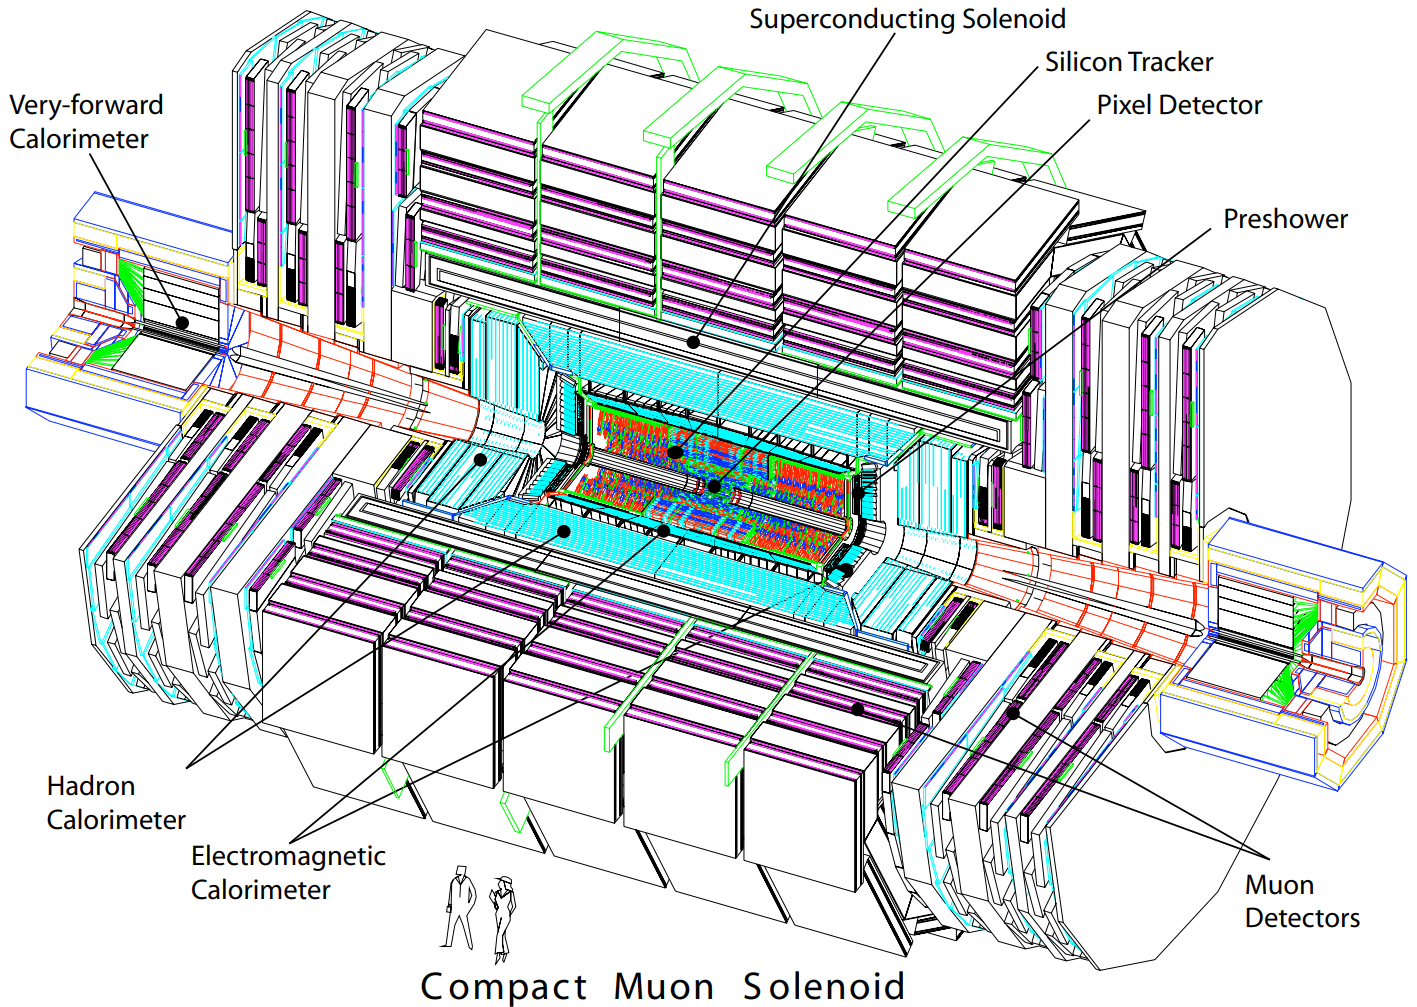
\includegraphics[width=0.98\textwidth]{Images/CMS.png}
	\captionof{figure}{Diagram of the CMS detector showing inner components (retrieved from~\parencite{Collaboration_2008})}\label{fig_cms}
\end{center}

The different sub-detectors are located concentrically in layers~\parencite{Collaboration_2008}. The inner most layer has a pixel detector made out of silicon, used for the reconstruction of primary and secondary vertices from electrically charged particles that decay promptly within this sub-detector volume. The pixel detector is followed by a sub-detector made of silicon strips, known as the tracker detector, used for the reconstruction of trajectories of electrically charged particles. Following the tracker detector, are found the electromagnetic (ECAL) and hadron (HCAL) calorimeters, used to measure both energy and direction of the particles undergoing electromagnetic and strong interactions, respectively. The ECAL detector is a modular device composed of lead-tugsten crystals, highly efficient to produce electromagnetic showers after interacting with charged particles. The emerging photons from the showers are measured using photo-diodes, that collect the light produced from the signal and convert it into an electric signal. This signal is then used by software tools to detect the energy and direction of the corresponding particles~\parencite{Collaboration_2008}. The ECAL is made of non magnetic materials such as copper and steel, which are characterized by heavy nuclei favoring strong interactions. Following a similar functioning as ECAL, hadronic particles enter the calorimeter, interact with the non-magnetic layers producing hadronic showers. These showers are then detected by plastic scintillators and their signals are transformed into electric pulses. These signals are then analyzed to estimate the energy and direction of the original particles~\parencite{Collaboration_2008}.

The next layer of the detector consists of a superconducting solenoid, which surrounds the previous sub-detectors. This solenoid is made of a niobum-titanium alloy that is refrigerated to $2 \mathrm{~K}$ by using liquid helium, producing a uniform magnetic field of $3.8 \mathrm{~T}$ inside the barrel~\parencite{Collaboration_2008}. This magnetic field is used to measure the momentum of electrically charged particles as it induces curvatures in their trajectories.

Finally, the last set sub-detectors conform the muon detector system. This system is made of three different detector technologies, that allow to reconstruct the trajectory of the muons with a fast trigger response, and are alternated with iron returning yokes of steel to enclose the magnetic field produced by the solenoid. The trigger is a date-filtering system composed of hardware and software algorithms, designed to collect interesting events from the proton-proton collisions. The muon detectors have a total of 1400 chambers distributed in 250 drift tubes, 540 cathode strip chambers that track the position of a muon and provide a trigger, as well as 610 resistive plate chambers that give a redundant trigger, which quickly decide over the event storage~\parencite{Collaboration_2008}.

% To do: ADD related with aceptance and efficiency in the barrel and endcaps.

Due to its cylindrical geometry, the CMS detector is divided into a central barrel region and two forward endcaps, which define the detector acceptance in terms of the pseudorapidity. The barrel region provides coverage for $|\eta| \lesssim 1.5$, while the endcap regions extend the acceptance up to $1.5\lesssim|\eta| \lesssim 2.5$ for most subsystems~\parencite{Collaboration_2008}. 

This geometrical segmentation impacts the overall detection efficiency. For example, the pixel and silicon strip trackers are more efficient in the barrel, where multiple tracking layers are crossed perpendicularly by particles. In the endcaps, particles cross detector layers at shallow angles, leading to reduced hit multiplicity and, consequently, lower tracking efficiency and resolution. Similar considerations apply to the ECAL and HCAL subsystems, where the granularity and material budget have been optimized to compensate for the non-uniform geometry, maintaining energy resolution across $\eta$.

Muon identification and momentum reconstruction also exhibit regional differences. The drift tubes (DTs), which offer high spatial resolution, are only installed in the barrel, while cathode strip chambers (CSCs) and resistive plate chambers (RPCs) cover the endcap regions. The combination of technologies ensures redundancy and robust triggering throughout the full detector acceptance. However, due to the higher background levels and increased radiation in the endcaps, the performance of muon reconstruction tends to be better in the barrel. For muons (electrons), the assumed identification efficiency is 95\% (85\%), with a 0.3\% (0.6\%) mis-identification rate~\parencite{CMS-PAS-FTR-13-014,CMS_MUON_17001,CMS_EGM_17001}.

Following reference~\parencite{CMS_BTV2016}, we use a flat identification efficiency for $\bq$ jets of 70\% across the entire $\pt$ spectrum with misidentification rate of 1\%. These values correspond with the  ``medium working point'' of the CMS algorithm to identify $\bq$ jets, known as DeepCSV. We also explored the ``Loose'' (``Tight'') working point using an efficiency of 85\% (45\%) and mis-identification rate of 10\% (0.1\%). 

For the performance of $\tau_{\textrm{h}}$ identification in DELPHES, we consider the latest technique described in~\parencite{CMS_DeepTau}, which is based on a deep neural network (i.e. DeepTau) that combines variables related to isolation and $\tau$-lepton lifetime as input to identify different $\tau_{\textrm{h}}$ decay modes. Following~\parencite{CMS_DeepTau}, we consider three possible DeepTau ``working points'': (i) the ``Medium'' working point of the algorithm, which gives a 70\% $\tau_{\textrm{h}}$-tagging efficiency and 0.5\% light-quark and gluon jet mis-identification rate; (ii) the ``Tight'' working point, which gives a 60\% $\tau_{\textrm{h}}$-tagging efficiency and 0.2\% light-quark and gluon jet mis-identification rate; and (iii) the ``VTight'' working point, which gives a 50\% $\tau_{\textrm{h}}$-tagging efficiency and 0.1\% light-quark and gluon jet mis-identification rate. Similar to the choice of $\textrm{b}$-tagging working point, the choice of $\tau_{\textrm{h}}$-tagging working point is determined through an optimization process which maximizes discovery reach. The ``Medium'' working point was ultimately shown to provide the best sensitivity and therefore chosen for this study. 

// ...existing code...
\section{The Phenomenological Pipeline: From Theory to Observables}

The estimation of signal and background event yields is performed through a comprehensive Monte Carlo (MC) simulation pipeline. This approach, a cornerstone of high-energy physics research, enables robust studies of Beyond the Standard Model (BSM) scenarios by emulating the entire data collection and processing chain of a collider experiment. The key advantages of this methodology include:

\begin{itemize}
    \item The ability to perform automated calculations of theoretical quantities such as cross-sections and decay widths for complex processes.
    \item Conducting feasibility studies and optimizing analysis strategies prior to data acquisition.
    \item Estimating the efficiency of complex event selection criteria and the geometric acceptance of the detector.
    \item Predicting the rates and kinematical distributions of both irreducible and reducible background processes.
    \item Comparing and distinguishing between different theoretical hypotheses for a potential discovered signal.
\end{itemize}

The simulation workflow is modular, reflecting the logical progression from a theoretical Lagrangian to simulated detector-level observables. A schematic view of this pipeline is presented in Figure~\ref{fig:sim_workflow}. The process begins with the implementation of the theoretical model in \texttt{FeynRules} (v2.3.43)~\parencite{Christensen:2008py,Alloul:2013bka}. The Lagrangian of the new physics scenario, including all particle definitions, parameters, and interactions, is translated into a set of Feynman rules. The output is exported in the Universal FeynRules Output (UFO) format, a standard interoperable with modern matrix element generators.

This UFO module, accompanied by a parameter card defining the numerical values of all model parameters (masses, couplings, etc.), serves as input to the \texttt{MadGraph5\_aMC@NLO} (v3.5.7)~\parencite{Alwall:2014bza,Alwall:2014hca} framework. Within MadGraph, the hard scattering process is defined, and the corresponding matrix elements (ME) and Feynman diagrams are generated at leading order (LO) in QCD. For this analysis, proton-proton collisions are simulated at center-of-mass energies of $\sqrt{s}=13 \tev$ and $\sqrt{s}=13.6 \tev$, utilizing the NNPDF3.0 NLO~\parencite{NNPDF:2014otw} set of parton distribution functions (PDFs). This choice is motivated by its global fit accuracy and consistency for both LO and NLO simulations.

To accurately model processes featuring significant interference effects between the new physics signal (e.g., a $\zb'$ boson) and the Standard Model backgrounds, the full squared amplitude (often referred to as the Signal-Discriminated Events or SDE strategy) is employed for the phase-space integration. The \texttt{MadEvent} submodule then generates unweighted parton-level events, which are stored in the Les Houches Event (LHE) format, containing the four-momenta of all final-state particles. The generation is optimized through careful configuration of the \texttt{run\_card}, setting appropriate kinematic cuts on final-state partons to avoid wasting computational resources on events that would subsequently be rejected by the detector simulation.

Given the presence of additional jet radiation, the MLM matching scheme~\parencite{Alwall:2007fs} is applied to mitigate the double-counting of jet emission between the matrix element calculation and the subsequent parton shower. This ensures a smooth transition between the hard process and softer radiative effects.

The parton-level LHE events are then passed to \texttt{PYTHIA} (v8.2.44)~\parencite{Sjostrand:2014zea} for the modeling of QCD and QED radiation (parton showering), hadronization, and particle decays. This step translates the colored partons into stable, color-singlet hadrons and resonances that form the observable final state. The resulting events, which include a full list of generator-level particles, are saved in the HepMC2 format.

Detector effects are simulated using \texttt{DELPHES} (v3.4.2)~\parencite{deFavereau:2013fsa}, a fast parametric detector simulation framework. The \texttt{delphes\_card\_CMS.tcl} configuration card is used to emulate the response of the CMS detector, including the geometric acceptance, tracking efficiency, calorimeter energy resolution and segmentation, and magnetic field. Key reconstruction algorithms are applied within DELPHES:
\begin{itemize}
    \item Jets are clustered from calorimeter towers using the anti-$k_t$ algorithm~\parencite{Cacciari:2008gp} with a distance parameter of $R=0.4$, and $b$-tagging is simulated based on the efficiency and mis-tag rate of the CMS performance.
    \item Muons and electrons are identified with efficiency maps that are functions of $p_T$ and $\eta$.
    \item The missing transverse energy (MET) is calculated from the negative vector sum of all reconstructed particle momenta.
\end{itemize}
The final output, containing reconstructed physics objects (jets, leptons, MET), is stored in ROOT format~\parencite{Brun:1997pa}.

At this stage, the analysis of the simulated samples converges with the methodology applied to real collider data. The subsequent steps involve applying event selection criteria, calibrating and scaling the reconstructed objects (e.g., applying Jet Energy Corrections), and performing statistical interpretation. The reliability of the simulation is validated by comparing the modeling of well-known Standard Model processes (e.g., Drell-Yan, $t\bar{t}$ production) against published results and data-driven control regions. Dominant theoretical systematic uncertainties, such as those arising from the choice of factorization and renormalization scales, PDF variations, and parton shower modeling, are evaluated and propagated through the analysis.


\section{Measurement of the Power of an Analysis}
\label{sec:power_analysis}

In high-energy physics experiments, data is often discretized into bins (e.g., histograms of collision events versus energy or momentum) to test competing hypotheses. The fundamental framework compares two scenarios: the \textit{null hypothesis} ($H_0$), representing background-only processes ($b_i$ in each bin $i$), and the \textit{alternative hypothesis} ($H_1$), including both signal and background ($s_i + b_i$). Given the Poissonian nature of event counts $n_i$, the likelihood for observing the data under each hypothesis is:
\begin{equation}
    \mathcal{L}(n_i \mid \lambda_i) = \frac{e^{-\lambda_i} \lambda_i^{n_i}}{n_i!}, \quad \text{where } \lambda_i = 
    \begin{cases}
        b_i & \text{for } H_0, \\
        s_i + b_i & \text{for } H_1.
    \end{cases}
\end{equation}
The Neyman-Pearson lemma~\parencite{NeymanPearson1933} provides a rigorous framework for hypothesis testing by establishing that the \textit{likelihood ratio} $Q = \mathcal{L}(\text{data} \mid H_1)/\mathcal{L}(\text{data} \mid H_0)$ is the most powerful test statistic for distinguishing between two simple hypotheses, $H_0$ and $H_1$. This forms the basis for quantifying the evidence for new physics signals against known backgrounds. For binned analyses in particle physics, we define the likelihood ratio $Q_i$ for each bin $i$ as,
\begin{equation}
Q_i = \frac{\mathcal{L}(n_i \mid s_i + b_i)}{\mathcal{L}(n_i \mid b_i)} = e^{-s_i} \left( 1+\frac{s_i}{b_i} \right)^{n_i},
\end{equation}
where $n_i$ is the observed event count, $s_i$ the expected signal, and $b_i$ the expected background in bin $i$. 


The test statistic for the full analysis is constructed as the product of individual bin likelihood ratios:
\begin{equation}
Q = \prod_{i=1}^{N} Q_i,
\end{equation}
where $N$ is the total number of bins. Under this formulation, each bin is treated as an independent experiment, allowing us to analyze the data in a modular way. This is particularly useful when combining results from multiple search channels or energy ranges. If we take the logarithm of the likelihood ratio this property turns into an additive form and, by the Wilks' theorem~\parencite{Wilks1938}, the asymptotic distribution of the test statistic $-2\ln Q$ under the background-only hypothesis ($H_0$) follows the $\chi^2$ distribution facilitating p-value calculations and hypothesis testing. So, for convenience and connection to asymptotic distributions, we consider the logarithmic form:
\begin{equation}
-2\ln Q = -2 \sum_{i=1}^{N} \ln Q_i = 2\sum_{i=1}^{N}\left[s_i - n_i \ln\left(1 + \frac{s_i}{b_i}\right)\right].
\end{equation}
Then, the practical implementation of the Neyman-Pearson lemma in particle physics leads to the definition of a test statistic $t$ that quantifies the evidence for a signal against the background-only hypothesis, constructed as
\begin{equation}
t=-2\ln Q = \sum_{i=1}^{N} \left[2s_i - 2n_i w_i\right]
\end{equation}
where $N$ is the total number of bins and $w_i = \ln(1 + s_i/b_i)$ is the optimal weight for bin $i$.

The discovery significance $\kappa$ quantifies the statistical separation of $t$ if $n$ is distributed according to the background-only hypothesis ($H_0$) versus the signal-plus-background hypothesis ($H_1$), normalized by the standard deviation of the $H_1$ distribution,
\begin{equation}
\kappa = \frac{\braket{t}_{H_0} - \braket{t}_{H_1}}{\sigma_{H_1}}.
\end{equation}
The expected behavior differs under the signal-plus-background ($H_1$) and background-only ($H_0$) hypotheses:

\begin{itemize}
	\item \textbf{Under $H_1$ ($n_i \sim \text{Pois}(s_i + b_i)$)}:
	\begin{equation}
	\langle -2\ln Q \rangle_{s+b} = \sum_i \left[2s_i - 2(s_i + b_i)w_i\right]
	\implies \sigma^2_{s+b} = 4\sum_i (s_i + b_i) w_i^2.
	\end{equation}

	\item \textbf{Under $H_0$ ($n_i \sim \text{Pois}(b_i)$)}:
	\begin{equation}
	\langle -2\ln Q \rangle_{b} = \sum_i \left[2s_i - 2b_i w_i\right]
	\implies \sigma^2_{b} = 4\sum_i b_i w_i^2
	\end{equation}
\end{itemize}
Substituting in $\kappa$ gives a useful expression for the discovery significance,
\begin{align}
\kappa = \frac{\sum s_i w_i}{\sqrt{\sum (s_i + b_i) w_i^2}}
\end{align}
It quantifies the separation between the signal+background ($s+b$) and background-only hypotheses in units of standard deviations ($\sigma$), where $\kappa = 5$ corresponds to the traditional $5\sigma$ discovery threshold, $\kappa =3$ to a $3\sigma$ evidence to the traditional anomaly detection threshold, and $\kappa = 1.69$ to the $95\%$ confidence level (CL) exclusion limit.


This figure of merit automatically optimizes sensitivity through the logarithmic weights $w_i = \ln(1 + s_i/b_i)$, which naturally emphasize bins with either high signal-to-background ratios ($s_i/b_i$) or large absolute signal contributions ($s_i$). In asymptotic limits, $\kappa$ simplifies to intuitive forms: for dominant signals ($s_i \gg b_i$), it approaches $\sqrt{\sum s_i}$ (Poisson counting), while in background-dominated regimes ($s_i \ll b_i$), it reduces to an inverse-variance-weighted sum $\sum s_i / \sqrt{\sum b_i (s_i/b_i)^2}$. This dual behavior ensures optimal discrimination power across all signal regimes.

In practice, we must take into account systematic effects by incorporating nuisance parameters into the likelihood and profiling over uncertainty ranges. The power calculation can be extended to include systematic uncertainties by modifying the denominator as,
\begin{equation}
	\boxed{
	\kappa_{\text{sys}} = \frac{\sum_i s_i w_i}{\sqrt{\sum_i \left[(s_i + b_i) + \sigma^2_{\text{sys,signal},i} + \sigma^2_{\text{sys,bkg},i}\right] w_i^2}},
}
\label{eq:kappa_with_systematics}
\end{equation}
where $\sigma_{\text{sys}}$ terms represent the systematic uncertainties on signal and background predictions.
